\chapter{Benchmarking of Whole-Body Controllers for Locomotion on Rigid Environment\label{chapter:benchmarking_wbc}}

In Part~\ref{part:background} we introduced the background and the literature review of the thesis. Instead, this chapter presents the first contribution of the manuscript. 
Here, we present and compare several whole-body controllers for bipedal locomotion in a rigid environment. 
In particular, we specify the three-layer controller architecture presented in Figure~\ref{fig:three-layer}, as shown in Figure~\ref{fig:three-layer-wbc-benchmarking}. 
The \emph{trajectory optimization} layer is kept fixed with a unicycle-based planner~\citep{8594277} that generates the desired DCM and foot trajectories. The \emph{simplified model control layer}, instead, implements two types of controllers for the tracking of the DCM: an instantaneous and an MPC one. 
The content of the \emph{trajectory optimization} and \emph{simplified model control layer} is detailed in Chapter~\ref{chapter:simplified_benchmarking}. 
Finally, the \emph{whole-body QP control} ensures the tracking of the desired CoM and feet trajectories by considering the complete robot models. In this context, we first present a kinematics-based whole-body controller, and then we extend the framework to consider the robot dynamics. Thanks to the modularity of the two problems, it is possible to exchange the two implementations depending on the low-level control interfaces available on the robot. 
The several combinations of the control architecture along with the simplified model controllers presented in Chapter~\ref{chapter:simplified_benchmarking} are compared on the iCub humanoid robot v2.7 -- see Section~\ref{sec:icub2.7}.
\par 
The chapter is organized as follows. Section~\ref{sec:ik_qp} presents the kinematics-based whole-body QP control layer. Section~\ref{sec:dynamics_QP} details the dynamics-based whole-body controller. Section~\ref{sec:wbc_experimental_results} presents the experimental validation of the
proposed approach and shows an explanatory table comparing the different control approaches. Finally, Section~\ref{sec:wbc_conclusion} concludes the chapter.

The content of this chapter appears partially in:
\begin{leftbar}
	\begin{quote}%
		\bibentry{8625025} \vspace{5mm}\newline 
		\bibentry{Romualdi2020ARobots} \vspace{5mm} \newline
		\begin{tabular}{c p{10.0cm}}
			     Video & \href{https://www.youtube.com/watch?v=FIqwAO71Fc4}{\texttt{https://www.youtube.com/watch?v=FIqwAO71Fc4}} \\
			     GitHub &  \href{https://github.com/robotology/walking-controllers}{\texttt{robotology/walking-controllers}} 
		\end{tabular}
	\end{quote}
\end{leftbar}

\begin{figure}[t]
    \centering
    \includegraphics{chapter_wbc_benchmarking/figures/three-layer.tikz}
    \caption[The three layer controller architecture for bipedal locomotion in rigid environment]{The control architecture is composed of three layers: the \emph{trajectory optimization}, the \emph{simplified model control}, and the \emph{whole-body control}. The middle and the other layers are described in Chapter~\ref{chapter:simplified_benchmarking}.
    \label{fig:three-layer-wbc-benchmarking}}
\end{figure}

\section{Kinematics based whole-body QP control layer\label{sec:ik_qp}}
The goal of the kinematics-based whole-body QP control layer is to ensure the tracking of a set of kinematic quantities considering the robot's kinematics. The proposed controller computes the desired robot generalized mixed representation velocity ${}^{B[\mathcal{I}]}\nu$~\eqref{eq:mixed_generalized_robot_velocity}, where $B[\mathcal{I}] = (o_B, [\mathcal{I}])$ is a frame placed on the robot base and oriented as the inertial frame $\mathcal{I}$.
 We formulate the control problem using the stack of tasks approach. We achieve the control objective by framing the controller as a constrained optimization problem where the low priority tasks are embedded in the cost function, while the high priority tasks are treated as constraints. A similar approach has also been presented in~\citep{Khudher2016QuadraticConstraints,Rapetti2020Model-BasedKinematics,Kanoun2011KinematicTask}, it is important to recall that other strategies are available to solve the kinematics control problem, in this context it is worth mentioning~\citep{Sciavicco1988,Goldenberg1985ARobots,Buss2005SelectivelyKinematics}.
\par
In the next section, we present the set of low and high priority tasks. For the sake of clarity, we denote the generalized mixed robot velocity ${}^{B[\mathcal{I}]}\nu$ as $\nu$.

\subsection{Low and high priority tasks\label{sec:ik_tasks}}
What follows presents the tasks required to evaluate the desired generalized robot velocity, $\nu$. We denote by $\Psi$ the equality task and by $\Phi$ the inequality task.

\subsubsection{Centroidal momentum task}
The centroidal momentum, denoted with ${}_{\bar{G}} h \in \mathbb{R}^6$, is the aggregate linear and angular momentum of each robot link referred to the center of mass (CoM) of the robot ${}_{\bar{G}} h^\top =\begin{bmatrix} {}_{\bar{G}} h^{p^\top} &{}_{\bar{G}} h^{\omega^\top} \end{bmatrix}$ -- Section~\ref{sec:centroidal-dynamics}. It is worth recalling that the centroidal momentum can be factorized as follows~\eqref{eq:cmm_intro}
\begin{equation}\label{eq:wbc_cmm}
	{}_{\bar{G}} h = J_\text{CMM} \nu,
\end{equation}
where $J_\text{CMM}$ is the centroidal momentum matrix~\citep{orin08,Orin2013}.
In order to set a desired centroidal momentum trajectory, we specify the following task:
\begin{equation}
    \label{eq:ik_cm_task}
    \Psi_h = {}_{\bar{G}} h^* - J_\text{CMM} \nu,
\end{equation}
where the desired linear centroidal momentum is often chosen to guarantee the tracking of the desired center of mass trajectory $x^\text{ref}_\text{CoM}(t)$
\begin{equation}
\label{eq:ik_h_p_star}
    {}_{\bar{G}} h^{p^*} = m \left[\dot{x}^\text{ref}_\text{CoM} + K_\text{CoM} (x^\text{ref}_\text{CoM} - x_\text{CoM})\right].
\end{equation}
Here $K_\text{CoM}$ is a positive matrix.
The desired angular momentum ${}_{\bar{G}} h^{\omega^*}$ is often set equal to zero, i.e., ${}_{\bar{G}} h^{\omega^*} = 0_{3\times1}$.
\par
The centroidal momentum task is often split into the linear and angular centroidal momentum tasks. The linear centroidal momentum task, denoted with $\Psi_\text{CoM}$, is:
\begin{IEEEeqnarray}{ll}
\phantomsection \label{eq:ik_com_task} \IEEEyesnumber \IEEEyessubnumber*
    \Psi_\text{CoM} &= \begin{bmatrix} I_3 & 0_{3\times3} \end{bmatrix} \Psi_h \\
    &= {}_{\bar{G}} h^{p^*} - \begin{bmatrix} I_3 & 0_{3\times3} \end{bmatrix} J_\text{CMM} \nu \\
     &= {}_{\bar{G}} h^{p^*} - J_{\text{CMM}_p} \nu
\end{IEEEeqnarray}
where ${}_{\bar{G}} h^{p^*}$ is chosen as~\eqref{eq:ik_h_p_star} and $J_{\text{CMM}_p}$ is the matrix composed of the first three rows of $J_{\text{CMM}}$. Similarly, we introduce the angular momentum task:
\begin{IEEEeqnarray}{ll}
\phantomsection \IEEEyesnumber \IEEEyessubnumber*
\label{eq:ik_acm_task}
    \Psi_{h^{\omega}} &= \begin{bmatrix}  0_{3\times3} & I_3  \end{bmatrix} \Psi_h \\
    &= {}_{\bar{G}} h^{\omega^*} - \begin{bmatrix} 0_{3\times3} & I_3  \end{bmatrix} J_\text{CMM} \nu \\
     &= {}_{\bar{G}} h^{\omega^*} - J_{\text{CMM}_\omega} \nu,
\end{IEEEeqnarray}
where $J_{\text{CMM}_\omega}$ is the matrix composed of the last three rows of $J_{\text{CMM}}$.

\subsubsection{Cartesian task}
While walking, we often require some of the robot link frames to have a specific position and orientation with respect to the inertial frame. To accomplish this task, we recall that given a frame $L$, its velocity expressed in mixed representation, denoted as ${}^{L[\mathcal{I}]}\mathrm{v}_{\mathcal{I},L}$, is given by
\begin{equation}
    {}^{L[\mathcal{I}]}\mathrm{v}_{\mathcal{I},L} = J_{L} \nu
\end{equation}
where $J_{L}$ is the mixed velocity Jacobian of the link $L$~\eqref{eq:mixed-link-velocity}.
To ask for a desired Cartesian trajectory ${}^\mathcal{I} H_L^\text{ref} = (p_L^\text{ref}, {}^\mathcal{I} R_L^\text{ref}) \in \mathbb{R}^3 \times \SO(3)$, we specify the following task
\begin{equation}
\label{eq:ik_se3_task}
    \Psi_{L_{\SE(3)}} = {}^{L[\mathcal{I}]}\mathrm{v}^*_{\mathcal{I},L} - J_{L} \nu
\end{equation}
where $ {}^{L[\mathcal{I}]}\mathrm{v}^*_{\mathcal{I},L} =\begin{bmatrix}
\dot{p}_L^{*^\top} & {}^\mathcal{I}\omega^{*^\top}_{\mathcal{I},L}
\end{bmatrix} ^\top $ is chosen as
\begin{IEEEeqnarray}{c}
\phantomsection \IEEEyesnumber \IEEEyessubnumber*
\dot{p}_L^{*} = \dot{p}_L^\text{ref} + K_{L_p}(p_L^\text{ref} - p_L) \label{eq:ik_se3_task_velocity_R3} \\
{}^\mathcal{I}\omega^{*}_{\mathcal{I},L} = {}^\mathcal{I}\omega^\text{ref}_{\mathcal{I},L} +  K_{L_\omega} \Log\left({}^\mathcal{I} R_L^\text{ref} \;\; {}^\mathcal{I} R_L^\top\right). \label{eq:ik_se3_task_velocity_so3}
\end{IEEEeqnarray}
Here $K_{L_p}$ and $K_{L_\omega}$ are two positive matrices.
By such a particular choice of the desired velocity~\eqref{eq:ik_se3_task_velocity_so3}, it is possible to guarantee almost-global stability and convergence of ${}^\mathcal{I}R _{L}$ to ${}^\mathcal{I}R _{L}^\text{ref}$~\citep{Olfati-Saber:2001:NCU:935467}.
\par
Starting from the definition of the $\SE(3)$ task~\eqref{eq:ik_se3_task}, we introduce the positional and rotational tasks for the frame $L$, respectively, denoted as $\Psi_{L_{\mathbb{R}^3}}$ and $\Psi_{L_{\SO(3)}}$.
The positional task $\Psi_{L_{\mathbb{R}^3}}$ is just a projection of the $\SE(3)$ task $\Psi_{L_{\SE(3)}}$ as:
\begin{IEEEeqnarray}{ll}
\phantomsection \label{eq:ik_r3_task}
 \IEEEyesnumber \IEEEyessubnumber*
\Psi_{L_{\mathbb{R}^3}} &= \begin{bmatrix}
    I_3 & 0_{3\times3} 
    \end{bmatrix}\Psi_{L_{\SE(3)}} \\
    &= \dot{p}^*_L - \begin{bmatrix}
    I_3 & 0_{3\times3} 
    \end{bmatrix} J_L \nu \\
     &= \dot{p}^*_L -  J_{L_p} \nu,
\end{IEEEeqnarray}
where $\dot{p}^*_L$ is set as \eqref{eq:ik_se3_task_velocity_R3} and $J_{L_p}$ is the matrix composed of the first three rows of $J_{L}$.
Similarly, we define the $\SO(3)$ task as follows:
\begin{IEEEeqnarray}{ll}
\phantomsection \label{eq:ik_so3_task} \IEEEyesnumber \IEEEyessubnumber*
\Psi_{L_{\SO(3)}} &= \begin{bmatrix}
    0_{3\times3} & I_3 
    \end{bmatrix}\Psi_{L_{\SE(3)}} \\
    &= {}^\mathcal{I} \omega^*_{\mathcal{I},L} - \begin{bmatrix}
    0_{3\times3} & I_3 
    \end{bmatrix} J_L \nu \\
     &= {}^\mathcal{I} \omega^*_{\mathcal{I},L} -  J_{L_\omega} \nu.
\end{IEEEeqnarray}
${}^\mathcal{I} \omega^*_{\mathcal{I},L}$ is set as \eqref{eq:ik_se3_task_velocity_so3} and $J_{L_\omega}$ is the matrix composed of the last three rows of $J_{L}$.

\subsubsection{Joint regularization task}
In order to prevent the controller from providing solutions with huge joint variations, we introduce a regularization task for the joint variables. The task is achieved by asking for a desired joint velocity that depends on the error between the desired and measured joint values, such as:
\begin{equation}
    \label{eq:ik_s_task}
    \Psi_s = \dot{s}^* - \begin{bmatrix}
    0_{n\times6} & I_n 
    \end{bmatrix} \nu,
\end{equation}
where $n$ is equal to the robot actuated degrees of freedom and $\dot{s}^*$ is set equal to
\begin{equation}
    \dot{s}^* = \dot{s}^\text{ref} + K_s (s^\text{ref} - s).
\end{equation}
Here $s^\text{ref}$ is the desired joint configuration. $K_s$ is a positive define diagonal matrix.

\subsubsection{Joint limits task}
The feasibility of the joint position $s$ is generally guaranteed by means of a set of inequalities of the form 
\begin{equation}
\label{eq:ik_joint_limits}
    s^- \le s \le s^+,
\end{equation}
where $s^-$ and $s^+$ are respectively the lower and upper joints position limits. 
In the case of the kinematics-based whole-body controller, the joint values $s$ cannot be arbitrarily chosen. To overcome this issue, we substitute the joint position $s$ in~\eqref{eq:ik_joint_limits} with its discrete dynamics computed at time using the forward Euler method $t_0 + k \diff t$, i.e., $s(t_0 + (k+1) \diff t) = s_{k+1} = s_k + \diff t \dot{s}_k$:
\begin{equation}
\label{eq:ik_joint_limits_euler}
    s^- \le  s_k + \diff t \dot{s}_k \le s^+.
\end{equation}
Rearranging~\eqref{eq:ik_joint_limits_euler} we obtain the final formulation of the joint limits task
\begin{equation}
   \Phi_s :  \;\; \frac{s^-  -s}{\diff t} \le   \dot{s} \le \frac{s^+  -s}{\diff t}.
\end{equation}
where we remove the time dependency $k$.

\subsection{Quadratic programming problem\label{sec:ik_qp_problem}}
The control objective is achieved by transcribing the control problem as a constrained optimization problem considering the tasks presented in Section~\ref{sec:ik_tasks}.
We want to underline that given an equality task $\Psi$, it is always possible to consider it as a low or high priority task, or, in another word, as a term of the cost function or as an equality constraint. Consequently, this makes the kinematics based whole-body problem modular\footnote{The \texttt{QPInverseKinematics} class implemented in our framework exploits this modularity to customize the control problem: \href{https://github.com/ami-iit/bipedal-locomotion-framework/tree/v0.6.0/src/IK}{\texttt{https://github.com/ami-iit/bipedal-locomotion-framework/tree/v0.6.0/src/IK}}}. A different choice of the considered tasks and priorities allows one to obtain completely different robot behaviors. Given the above observation, we decide to present the specific implementation we consider in the experimental results -- Section~\ref{sec:wbc_experimental_results}.
\par
The tracking of the left and right foot poses are considered as high priority $\SE(3)$ tasks~\eqref{eq:ik_se3_task} and are denoted respectively as $\Psi_{L_{\SE(3)}}$ and $\Psi_{R_{\SE(3)}}$. We take into account the CoM tracking as a high priority task~\eqref{eq:ik_com_task}.
The torso orientation is considered as a low priority task $\SO(3)$ task~\eqref{eq:ik_so3_task} and we denote it with $\Psi_{T_{\SO(3)}}$. Furthermore, the joint postural condition~\eqref{eq:ik_s_task} is also added as a low priority task. Finally, we ask for a joint velocity $\dot{s}$ such that the inequality joint limits task~\eqref{eq:ik_joint_limits_euler} is satisfied.
\par
The above hierarchical control objectives can be cast into a whole-body optimization problem:
\begin{IEEEeqnarray}{CL}
\phantomsection \label{eq:ik_optimization} \IEEEyesnumber \IEEEyessubnumber*
\;\minimize\limits_{\nu} \; & \Psi_{T_{\SO(3)}}^\top \Lambda_T \Psi_{T_{\SO(3)}} + \Psi_{s}^\top \Lambda_s \Psi_{s} \label{eq:ik_optimization_cost} \\
\st & \Psi_{L_{\SE(3)}} = 0  \label{eq:ik_optimization_costraint_lf} \\
&  \Psi_{R_{\SE(3)}} = 0 \label{eq:ik_optimization_costraint_rf} \\
& \Psi_{\text{CoM}} = 0 \label{eq:ik_optimization_costraint_com} \\
& \Phi_s. \label{eq:ik_optimization_costraint_s}
\end{IEEEeqnarray}
Since the decision variable is the robot velocity $\nu$ and the tasks depend linearly on $\nu$, we transcribe the optimization problem~\eqref{eq:ik_optimization} into a quadratic programming problem (Section~\ref{sec:qp}) of the form: 
\begin{IEEEeqnarray}{CLL}
\phantomsection \IEEEyesnumber \IEEEyessubnumber*
\;\minimize\limits_{\nu} \;& \IEEEeqnarraymulticol{2}{C}{\nu ^\top H \nu + 2 g^\top \nu} \\
\st & A \nu \preceq b
\end{IEEEeqnarray}
The Hessian matrix $H$ and the gradient vector $g$ are evaluated from \eqref{eq:ik_optimization_cost}.
The constraint matrix and vector $A$ and $b$ are obtained from \eqref{eq:ik_optimization_costraint_lf},  \eqref{eq:ik_optimization_costraint_rf},  \eqref{eq:ik_optimization_costraint_com} and  \eqref{eq:ik_optimization_costraint_s}.
Using this formulation, the optimization problem can be solved using a standard numerical QP solver.

\subsection{Position and velocity controlled robot}
\label{subsubsec-pos-vel-control}
It is important to notice that the outcome of~\eqref{eq:ik_optimization} is (also) the robot joint velocity. When a robot velocity controller is available, one can set these joint velocities to the low-level robot controller. In this case, the \emph{*} quantities in the tasks (Section~\ref{sec:ik_tasks}) can be evaluated using the feedback from the robot sensors, and the robot is said to be \emph{velocity controlled}. On the other hand, if the robot velocity control is not available, one may integrate the outcome of~\eqref{eq:ik_optimization} to obtain desired joint position to be set to a low-level robot position controller. In this case, the \emph{*} quantities in~\eqref{eq:ik_optimization} can be evaluated using the desired integrated quantities instead of the sensor feedback, and~\eqref{eq:ik_optimization} behaves as an inverse kinematics module. Consequently, the robot is said to be \emph{position controlled}.

\section{Dynamics-based whole-body QP control layer} \label{sec:dynamics_QP}
The Dynamics-based whole-body QP control layer considers the dynamic model of the system to ensure the tracking of the desired trajectories. The proposed controller computes the desired robot joint torque $\tau$, the generalized mixed representation acceleration ${}^{B[\mathcal{I}]}\dot{\nu}$, and a set of desired spatial contact forces expressed in the mixed representation ${}_{\mathcal{C}_j[\mathcal{I}]}\mathrm{f}_j$. Here $B[\mathcal{I}] = (o_B, [\mathcal{I}])$ is a frame placed on the base of the robot and oriented as the inertial frame $\mathcal{I}$. On the other hand, $\mathcal{C}_j[\mathcal{I}] = (p_j, \mathcal{I})$ is the frame associated with the admissible contact (e.g. the foot) where $j\in\mathbb{N}$ such that $1\le j \le n_c$, with $n_c$ is the number of admissible contacts. The control problem is formulated using the stack of tasks approach. Similar to the kinematics based whole-body control layer (Section~\ref{sec:ik_qp}), the objective is achieved by transcribing the problem as a constrained optimization problem. We define the low priority tasks as terms of the cost function. While the high priority tasks are treated as constraints.
\par
An approach similar to the one presented in this section has been also described in~\citep{nava16,Dean-Leon2019Whole-BodySkin,Englsberger2018,DelPrete2016ImplementingSensors,Henze2016,Ramuzat2022PassiveMulti-Contact,Mesesan2019}
\par
In the next section, we present the set of low and high priority tasks. For the sake of clarity, we simplify the notation of the generalized mixed robot velocity and acceleration by dropping the superscript $B[\mathcal{I}]$. Furthermore the contact wrenches are stacked into a vector $\mathrm{f} = \begin{bmatrix}
{}_{\mathcal{C}_1[\mathcal{I}]}\mathrm{f}_1^\top & {}_{\mathcal{C}_2[\mathcal{I}]}\mathrm{f}_2^\top & \hdots & {}_{\mathcal{C}_{n_c}[\mathcal{I}]}\mathrm{f}_{n_c}^\top 
\end{bmatrix}^\top \in \mathbb{R}^{6 n_c }$

\subsection{Low and high priority tasks\label{sec:tsid_tasks}}
What follows presents the tasks required to define the control objectives. We denote by $\Psi$ the equality task and by $\Phi$ the inequality task.

\subsubsection{Centroidal momentum task}
Given a frame $\bar{G} = (x_\text{CoM},[\mathcal{I}])$, the centroidal momentum rate of change ${}_{\bar{G}} \dot{h}$ balances the external spatial force applied on the robot~\eqref{eq:centroidal_momentum_dynamics_mixed}:
\begin{equation}
    \label{eq:tsid_centroidal_dynamics}
    {}_{\bar{G}} \dot{{h}} = \sum_{j = 1}^{n_c} \begin{bmatrix}
	I_3 & {0}_{3\times 3} \\
	\left({p}_j - {x}_\text{CoM}\right)\times & I_3 
	\end{bmatrix} {}_{\mathcal{C}_j[\mathcal{I}]}\mathrm{f}_j + m \bar{g},
\end{equation}
where $\bar{g} = \begin{bmatrix} 0&0&-g&0&0&0 \end{bmatrix}^\top$ is the 6D gravity acceleration vector.  Rearranging Equation~\eqref{eq:tsid_centroidal_dynamics}, we obtain
\begin{IEEEeqnarray}{LL}
\phantomsection \IEEEyesnumber \IEEEyessubnumber*
 {}_{\bar{G}} \dot{{h}} &= \begin{bmatrix}
	I_3 & {0}_{3\times 3} & \hdots & I_3 & {0}_{3\times 3} \\
	\left({p}_1 - {x}_\text{CoM}\right)\times & I_3 & \hdots & \left({p}_{n_c} - {x}_\text{CoM}\right)\times & I_3 
	\end{bmatrix} \mathrm{f} + m \bar{g} \\
	&= A_c \mathrm{f} + m\bar{g}.
\end{IEEEeqnarray}
To ask for a desired centroidal momentum trajectory, we specify the following task:
\begin{equation}
    \Phi_h = {}_{\bar{G}} \dot{{h}}^* - A_c \mathrm{f} - m\bar{g}.
\end{equation}
We set the desired linear centroidal momentum rate of change to guarantee the tracking of the desired center of mass trajectory $x_\text{CoM}^\text{ref}(t)$ as 
\begin{equation}
\label{eq:tsid_h_p_star}
   {}_{\bar{G}} \dot{{h}}^{p^*} = m\left[ \ddot{x}^\text{ref}_\text{CoM} +K^d_\text{CoM} (\dot{x}^\text{ref}_\text{CoM} - \dot{x}_\text{CoM}) + K^p_\text{CoM}({x}^\text{ref}_\text{CoM} - {x}_\text{CoM})   \right].
\end{equation}
Here $K^p_\text{CoM}$ and $K^d_\text{CoM}$ are positive define diagonal matrices. On the other hand,  the desired angular momentum rate of change ${}_{\bar{G}} \dot{{h}}^{\omega^*}$ is given by
\begin{equation}
\label{eq:tsid_h_omega_star}
      {}_{\bar{G}} \dot{{h}}^{\omega^*} = {}_{\bar{G}} \dot{{h}}^{\omega^\text{ref}} + K_{h^\omega} \left({}_{\bar{G}} {{h}}^{\omega^\text{ref}} - {}_{\bar{G}} {{h}}^{\omega}\right),
\end{equation}
where $ K_{h^\omega} > 0$. If a high-level whole-body planner is available, for instance \citep{carpentier2016versatile}, ${{h}}^{\omega^\text{ref}}$ is chosen to satisfy~\eqref{eq:cmm_intro}
\begin{equation}
    {}_{\bar{G}} h^{\omega^\text{ref}} = J_{\text{CMM}_\omega}^\text{pl} {\nu}^\text{pl},
\end{equation}
where the superscript \emph{pl} indicates that the quantity is computed by the high-level planner. 
Another common choice is to set the desired angular momentum equal to zero, i.e., ${{h}}^{\omega^\text{ref}} = 0_{3\times1}$
\par
Similar to the kinematics-based controller case, the centroidal momentum task is often divided into linear and angular centroidal momentum tasks. The linear task, denoted by $\Psi_\text{CoM}$ is given by
\begin{IEEEeqnarray}{ll}
\phantomsection \label{eq:tsid_com_task} \IEEEyesnumber \IEEEyessubnumber*
    \Psi_\text{CoM} &= \begin{bmatrix} I_3 & 0_{3\times3} \end{bmatrix} \Psi_h \\
    &= {}_{\bar{G}} \dot{h}^{p^*} - \begin{bmatrix} I_3 & 0_{3\times3} \end{bmatrix} A_c \mathrm{f} - mg \\
     &= {}_{\bar{G}} \dot{h}^{p^*} - A_{c_p} \mathrm{f} - mg
\end{IEEEeqnarray}
where ${}_{\bar{G}} \dot{h}^{p^*}$ is chosen as~\eqref{eq:tsid_h_p_star} and $ A_{c_p}$ is the matrix composed of the first three rows of $ A_{c}$. The angular momentum task $\Psi_{h^{\omega}}$ is 
\begin{IEEEeqnarray}{ll}
\phantomsection \IEEEyesnumber \IEEEyessubnumber*
\label{eq:tsid_acm_task}
    \Psi_{h^{\omega}} &= \begin{bmatrix}  0_{3\times3} & I_3  \end{bmatrix} \Psi_h \\
    &= {}_{\bar{G}} \dot{h}^{\omega^*} - \begin{bmatrix} 0_{3\times3} & I_3  \end{bmatrix} A_c \mathrm{f} \\
     &= {}_{\bar{G}} \dot{h}^{\omega^*} - A_{c_\omega} \mathrm{f}.
\end{IEEEeqnarray}
${}_{\bar{G}} \dot{h}^{\omega^*}$ is set equal to \eqref{eq:tsid_h_omega_star}. $A_{c_\omega}$ is the matrix composed of the last three rows of $A_{c}$.

\subsubsection{Cartesian task}
While walking, we often require some of the robot link frames to have a specific position and orientation with respect to the inertial frame. To accomplish this task, we recall that given a frame $L$, its acceleration expressed in mixed representation, denoted as ${}^{L[\mathcal{I}]}\dot{\mathrm{v}}_{\mathcal{I},L}$, is given by
\begin{equation}
    {}^{L[\mathcal{I}]}\dot{\mathrm{v}}_{\mathcal{I},L} = J_{L} \dot{\nu} + \dot{J}_{L} {\nu},
\end{equation}
where $J_{L}$ is the mixed velocity Jacobian of the link $L$~\eqref{eq:mixed-link-velocity} and $\dot{J}_{L}$ its derivative. 
To follow a desired Cartesian trajectory ${}^\mathcal{I} H_L^\text{ref} = (p_L^\text{ref}, {}^\mathcal{I} R_L^\text{ref}) \in \mathbb{R}^3 \times \SO(3)$, we specify the following task:
\begin{equation}
\label{eq:tsid_se3_task}
    \Psi_{L_{\SE(3)}} =  {}^{L[\mathcal{I}]}\dot{\mathrm{v}}_{\mathcal{I},L}^* - J_{L} \dot{\nu} - \dot{J}_{L} {\nu},
\end{equation}
where $ {}^{L[\mathcal{I}]}\dot{\mathrm{v}}^*_{\mathcal{I},L} =\begin{bmatrix}
\ddot{p}_L^{*^\top} & {}^\mathcal{I}\dot{\omega}^{*^\top}_{\mathcal{I},L}
\end{bmatrix} ^\top $ is chosen as~\footnote{An efficient implementation of the controller is available at \href{https://github.com/ami-iit/lie-group-controllers}{\texttt{https://github.com/ami-iit/lie-group-controllers}}.}
\begin{IEEEeqnarray}{c}
\phantomsection \label{eq:tsid_se3_task_velocity} \IEEEyesnumber \IEEEyessubnumber*
\ddot{p}_L^{*} = \ddot{p}_L^\text{ref} +  K_{L_p}^d(\dot{p}_L^\text{ref} - \dot{p}_L) +  K_{L_p}^p(p_L^\text{ref} - p_L) \label{eq:tsid_se3_task_velocity_R3} \\
{}^\mathcal{I}\dot{\omega}^{*}_{\mathcal{I},L} = {}^\mathcal{I}\dot{\omega}^\text{ref}_{\mathcal{I},L} + K_{L_\omega}^d  ( {}^\mathcal{I}\omega^\text{ref}_{\mathcal{I},L} -  {}^\mathcal{I}\omega_{\mathcal{I},L}) +  K_{L_\omega}^p \Log\left({}^\mathcal{I} R_L^\text{ref} \;\; {}^\mathcal{I} R_L^\top\right). \label{eq:tsid_se3_task_velocity_so3}
\end{IEEEeqnarray}
Here $K_{L_p}^p$, $K_{L_p}^d$, $K_{L_\omega}^p$ and $K_{L_\omega}^d$ are positive defined matrices.
\par
Starting from the definition of the $\SE(3)$ task~\eqref{eq:tsid_se3_task}, we introduce the positional and rotational tasks for the frame $L$, respectively, denoted as $\Psi_{L_{\mathbb{R}^3}}$ and $\Psi_{L_{\SO(3)}}$:
\begin{IEEEeqnarray}{ll}
\phantomsection \label{eq:tsid_r3_task}
 \IEEEyesnumber \IEEEyessubnumber*
\Psi_{L_{\mathbb{R}^3}} &= \begin{bmatrix}
    I_3 & 0_{3\times3} 
    \end{bmatrix}\Psi_{L_{\SE(3)}} \\
    &= \ddot{p}^*_L - \begin{bmatrix}
    I_3 & 0_{3\times3} 
    \end{bmatrix} \left(J_L \dot{\nu}  + \dot{J}_L \nu  \right) \\
     &= \ddot{p}^*_L -  J_{L_p} \dot{\nu}  - \dot{J}_{L_p} \nu,
\end{IEEEeqnarray}
\begin{IEEEeqnarray}{ll}
\phantomsection \label{eq:tsid_so3_task} \IEEEyesnumber \IEEEyessubnumber*
\Psi_{L_{\SO(3)}} &= \begin{bmatrix}
    0_{3\times3} & I_3 
    \end{bmatrix}\Psi_{L_{\SE(3)}} \\
    &= {}^\mathcal{I} \dot{\omega}^*_{\mathcal{I},L} - \begin{bmatrix}
    0_{3\times3} & I_3 
    \end{bmatrix} \left(J_L \dot{\nu}  + \dot{J}_L \nu  \right) \\
     &= {}^\mathcal{I} \dot{\omega}^*_{\mathcal{I},L} -  J_{L_\omega} \dot{\nu}  - \dot{J}_{L_\omega} \nu.
\end{IEEEeqnarray}
$\ddot{p}^*_L$ is given by \eqref{eq:tsid_se3_task_velocity_R3}, while ${}^\mathcal{I} \dot{\omega}^*_{\mathcal{I},L}$ is obtained from \eqref{eq:tsid_se3_task_velocity_so3}. $J_{L_p}$ and $J_{L_\omega}$ are, respectively, the matrices composed of the first and last three rows of $J_{L}$.


\subsubsection{Floating base dynamics task}
To whole-body control layer often considers the base~\eqref{eq:robot_dynamics_base} and joint dynamics~\eqref{eq:robot_dynamics_joints} as a set of high priority tasks. In this context, we define the base dynamics task as 
\begin{equation}
    \label{eq:tsid_base_dyn_task}
    \Psi_{\text{dyn}_\nu} =  h_{\nu} + M_{\nu}\dot{\nu} - J_{\mathcal{C}_\nu}^\top \mathrm{f}.
\end{equation}
On the other hand, the joint dynamics task is given by
\begin{equation}
    \label{eq:tsid_joint_dyn_task}
    \Psi_{\text{dyn}_s} =  h_{s} +  M_{s}(q) \dot{\nu} - \tau - J_{\mathcal{C}_s}^\top \mathrm{f},
\end{equation}
where the subscript $\nu$ refers to the first 6 rows of the matrix, while $s$ to the last $n$ rows, with $n$ the number of actuated degrees of freedom of the system. 

\subsubsection{Joint regularization task}
To prevent the controller from providing solutions with huge joint variations, we introduce a regularization tasks for the joint variables. The task is achieved by asking for a desired joint velocity that depends on the error between the desired and measured joint values, such as:
\begin{equation}
    \label{eq:tsid_s_task}
    \Psi_s = \ddot{s}^* - \begin{bmatrix}
    0_{n\times6} & I_n 
    \end{bmatrix} \dot{\nu},
\end{equation}
$\ddot{s}^*$ is equal to
\begin{equation}
    \ddot{s}^* = \ddot{s}^\text{ref} + k_s^d (\dot{s}^\text{ref} - \dot{s}) + k_s^p (s^\text{ref} - s).
\end{equation}
Here $s^\text{ref}$ is the desired joint configuration trajectory and is often set constant, i.e. $s^\text{ref}(t) = \bar{s}$.


\subsubsection{Local ZMP task}
Given a desired ZMP position expressed in the ${\mathcal{C}_j[\mathcal{I}]}$ frame, we want to define a task such that the desired contact force in $\mathcal{C}_j$ generates ${}^{\mathcal{C}_j[\mathcal{I}]} x_{\text{ZMP}_j}$. We now recall that, given a 6D force ${}_{\mathcal{C}_j[\mathcal{I}]} \mathrm{f}_j$, the ZMP, if exists, is given by~\citep{vukobratovic2004zero}
\begin{equation}
    \label{eq:tsid_local_zmp_definition}
   {}^{\mathcal{C}_j[\mathcal{I}]} x_{\text{ZMP}_j} = 
   \begin{bmatrix}
   -\frac{{}_{\mathcal{C}_j[\mathcal{I}]} \mu_{j_y}}{{}_{\mathcal{C}_j[\mathcal{I}]} f_{j_z}} \\
   \frac{{}_{\mathcal{C}_j[\mathcal{I}]} \mu_{j_x}}{{}_{\mathcal{C}_j[\mathcal{I}]} f_{j_z}}
   \end{bmatrix}.
\end{equation}
Assuming that ${}_{\mathcal{C}_j[\mathcal{I}]} f_z \ne 0$, i.e., the contact is active, we rearrange Equation~\eqref{eq:tsid_local_zmp_definition} as
\begin{equation}
    \label{eq:tsid_local_zmp_definition_rearranged}
  {}_{\mathcal{C}_j[\mathcal{I}]} f_{z_j}  {}^{\mathcal{C}_j[\mathcal{I}]} x_{\text{ZMP}_j} = 
   \begin{bmatrix}
   -{}_{\mathcal{C}_j[\mathcal{I}]} \mu_{j_y} \\
   {}_{\mathcal{C}_j[\mathcal{I}]} \mu_{j_x}
   \end{bmatrix}.
\end{equation}
Considering~\eqref{eq:tsid_local_zmp_definition_rearranged}, we define the local ZMP task for the contact $\mathcal{C}_j$ as
\begin{equation}
    \Psi_{\text{ZMP}_j} = \left({}^{\mathcal{C}_j[\mathcal{I}]} x_{\text{ZMP}_j}^\text{ref} e_3^\top - 
    \begin{bmatrix}
        0& 0&0&0&-1&0 \\
        0& 0&0&1&0&0
    \end{bmatrix} \right) {}_{\mathcal{C}_j[\mathcal{I}]} \mathrm{f}_j.
\end{equation}

\subsubsection{Global ZMP task}
In the case all the robot contact lies on the same plane, for example, the robot is walking on a planar surface, it is possible to ask for a desired global ZMP, denoted with ${}^\mathcal{I}x_\text{ZMP}$ (please note that the suffix $j$ is not present in this case since the ZMP is considered as a global quantity and not strictly dependent to the contact).
Given $n_c$ coplanar contacts, we define the global ZMP as~\citep[Section~3.2.3]{Kajita2014IntroductionRobotics}:
\begin{equation}
\label{eq:tsid_zmp_global_def}
    {}^\mathcal{I}x_\text{ZMP} = \sum_{j=1}^{n_c} \frac{{}_{\mathcal{C}_j[\mathcal{I}]}f_{j_z}}{\sum_{i=1}^{n_c} {}_{\mathcal{C}_i[\mathcal{I}]}f_{i_z}}\left( p_j + {}^{\mathcal{C}_j[\mathcal{I}]}x_{\text{ZMP}_j}  \right).
\end{equation}
By combining~\eqref{eq:tsid_local_zmp_definition} with \eqref{eq:tsid_zmp_global_def} we obtain
\begin{equation}
    {}^\mathcal{I}x_\text{ZMP} = \sum_{j=1}^{n_c} \frac{{}_{\mathcal{C}_j[\mathcal{I}]}f_{j_z}}{\sum_{i=1}^{n_c} {}_{\mathcal{C}_i[\mathcal{I}]}f_{i_z}}\left( p_j + 
    \begin{bmatrix}
   -\frac{{}_{\mathcal{C}_j[\mathcal{I}]} \mu_{j_y}}{{}_{\mathcal{C}_j[\mathcal{I}]} f_{j_z}} \\
   \frac{{}_{\mathcal{C}_j[\mathcal{I}]} \mu_{j_x}}{{}_{\mathcal{C}_j[\mathcal{I}]} f_{j_z}}
   \end{bmatrix}  \right).
\end{equation}
Assuming that ${}_{\mathcal{C}_j[\mathcal{I}]}f_{j_z} > 0$ we define the global ZMP task as 
\begin{equation}
\label{eq:tsid_zmp_global_task}
    \Psi_{\text{ZMP}} = \left({}^{\mathcal{I}} x_{\text{ZMP}}^\text{ref}   \begin{bmatrix}
        e_3^\top & \hdots e_3^\top 
    \end{bmatrix}- 
    \begin{bmatrix}
        \Gamma_1 & \hdots \Gamma_{n_c}
    \end{bmatrix} \right)\mathrm{f},
\end{equation}
where $\Gamma_i\in \mathbb{R}^{2\times6}$ writes as
\begin{equation}
 \Gamma_i = \begin{bmatrix}
 0 & 0 & p_{i_x} & 0 & -1 & 0 \\
 0 & 0 & p_{i_y} & 1 & 0 & 0
 \end{bmatrix}.
\end{equation}


\subsubsection{Generic variable regularization task}
In order to prevent the controller from providing solutions with huge torque $\tau$ or contact force ${}_{\mathcal{C}_j[\mathcal{I}]}\mathrm{f}_j$, we introduce a regularization task of the form
\begin{equation}
    \label{eq:tsid_generic_regularization}
    \Psi_u = u^\text{ref} - u,
\end{equation}
where $u$ is either the joint torque $\tau$ or the contact force ${}_{\mathcal{C}_j[\mathcal{I}]}\mathrm{f}_j$.

\subsubsection{Feasibile contact force task}
The feasibility of the contact wrench ${}_{\mathcal{C}_j[\mathcal{I}]}\mathrm{f}_j$ is guaranteed by a set of inequality of the form:
\begin{equation}
  \Phi_{\mathrm{f}_j}: \;\;  \label{eq:tsid_contact_wrench_feasibility_constraint}
    A_{\mathcal{C}_j[\mathcal{I}]} \; {}_{\mathcal{C}_j[\mathcal{I}]}\mathrm{f}_j \le b.
\end{equation}
where $A_{\mathcal{C}_j[\mathcal{I}]}$ is a matrix that depends on the position of the robot joints and on the base pose.
\par
More specifically, ${}_{\mathcal{C}_j[\mathcal{I}]}\mathrm{f}_j$ must belong to the associated friction cone, while the position of the local CoP is constrained within the support polygon. 

\subsubsection{Joint limits task}
The feasibility of the joint position $s$ is generally guaranteed by means of a set of inequalities of the form 
\begin{equation}
\label{eq:tsid_joint_limits}
    s^- \le s \le s^+,
\end{equation}
where $s^-$ and $s^+$ are respectively the lower and upper joints position limits. 
In the case of dynamics-based whole-body controller, the joint values $s$ cannot be arbitrary chosen. To overcome this issue, we substitute the joint position $s$ in~\eqref{eq:tsid_joint_limits} with its second-order discrete dynamics computed at time $t_0 + k \diff t$ by applying the forward Euler method, i.e. $s(t_0 + (k+1) \diff t) = s_{k+1} = s_k + \diff t \dot{s}_k + 0.5 \diff t^2 \ddot{s}_k$:
\begin{equation}
\label{eq:tsid_joint_limits_euler}
    s^- \le  s_k + \diff t \dot{s}_k + \frac{1}{2} \diff t^2 \ddot{s}_k \le s^+.
\end{equation}
Rearranging~\eqref{eq:tsid_joint_limits_euler} we obtain the final formulation of the joint limits task
\begin{equation}
   \Phi_s :  \;\; 2 \frac{s^-  -s - \diff t \dot{s} }{\diff t^2} \le   \dot{s} \le 2 \frac{s^+  -s - \diff t \dot{s}}{\diff t^2}.
\end{equation}
where we remove the time dependency $k$.
\subsubsection{Feasible joint torque}
To guarantee feasible contact torque, we define the following inequality task
\begin{equation}
    \label{eq:tsid_joint_limits_torque_task}
    \Phi_\tau:\;\; \tau^{-} \le \tau \le \tau^+,
\end{equation}
where $\tau^{-}$ and $\tau^+$ represent the maximum negative and positive torque that the joints can produce. 

\subsection{Quadratic programming problem \label{sec:tsid_optimal_control_problem}}
The control objective is achieved by transcribing the control problem as a constrained optimization problem considering the tasks presented in Section~\ref{sec:tsid_tasks}.
Similarly to what we discussed for the kinematics-based whole-body controller in Section~\ref{sec:ik_qp}, an equality task $\Psi$ can always be considered as a lower or high priority task, or, in another word, as a term of the cost function or as an equality constraint. Consequently, this makes the dynamics based whole-body problem modular\footnote{The \texttt{QPTSID} class implemented in our framework exploits this modularity to customize the control problem: \href{https://github.com/ami-iit/bipedal-locomotion-framework/tree/v0.6.0/src/TSID}{\texttt{https://github.com/ami-iit/bipedal-locomotion-framework/tree/v0.6.0/src/TSID}}}. 
\par
From now on, we consider the following set of tasks.
The tracking of the left and right foot poses are considered as high priority $\SE(3)$ tasks~\eqref{eq:tsid_se3_task} and they are denoted respectively as $\Psi_{L_{\SE(3)}}$ and $\Psi_{R_{\SE(3)}}$. We take into account the CoM tracking as high priority task~\eqref{eq:tsid_com_task} and the global ZMP tracking~\eqref{eq:tsid_zmp_global_task}. We also consider the base~\eqref{eq:tsid_base_dyn_task} and the joint dynamics~\eqref{eq:tsid_joint_dyn_task} as high priority tasks. 
The torso orientation is implemented as a low priority task $\SO(3)$ task~\eqref{eq:tsid_so3_task} and we denote it with $\Psi_{T_{\SO(3)}}$. Furthermore, the joint postural condition~\eqref{eq:tsid_s_task} is also added as a low priority task. To minimize the joint torques and forces, we also add two regularization tasks~\eqref{eq:tsid_generic_regularization} denoted $\Psi_\tau$ and $\Psi_\mathrm{f}$. We also ask for a joint torque $\tau$ such that the inequality joint limits task~\eqref{eq:tsid_joint_limits_torque_task} is satisfied. Finally, to guarantee feasible contact forces for the left and right feet, we add the task~\eqref{eq:tsid_contact_wrench_feasibility_constraint}, denoted respectively as $\Phi_{\mathrm{f}_L}$ and $\Phi_{\mathrm{f}_R}$.
\par
The above hierarchical control objectives can be cast into a whole-body optimization problem:
\begin{IEEEeqnarray}{CL}
\phantomsection \label{eq:tsid_optimization} \IEEEyesnumber \IEEEyessubnumber*
\;\minimize\limits_{\dot{\nu}, \; \tau, \;\mathrm{f}} \; & \Psi_{T_{\SO(3)}}^\top \Lambda_T \Psi_{T_{\SO(3)}} + \Psi_{s}^\top \Lambda_s \Psi_{s} + \Psi_{\mathrm{f}}^\top \Lambda_\mathrm{f} \Psi_{\mathrm{f}} + \Psi_{\tau}^\top \Lambda_\tau \Psi_{\tau} \label{eq:tsid_optimization_cost} \\
\st & \Psi_{L_{\SE(3)}} = 0  \label{eq:tsid_optimization_costraint_lf} \\
&  \Psi_{R_{\SE(3)}} = 0 \label{eq:tsid_optimization_costraint_rf} \\
& \Psi_{\text{CoM}} = 0 \label{eq:tsid_optimization_costraint_com} \\
& \Psi_{\text{dyn}_\nu} = 0 \label{eq:tsid_optimization_costraint_dyn_base} \\
& \Psi_{\text{dyn}_s} = 0 \label{eq:tsid_optimization_costraint_dyn_s} \\
& \Psi_{\text{ZMP}} = 0 \label{eq:tsid_optimization_costraint_zmp} \\
& \Phi_s \label{eq:tsid_optimization_costraint_s}  \\
& \Phi_\tau \label{eq:tsid_optimization_costraint_tau} \\
&\Phi_{\mathrm{f}_L} \\
&\Phi_{\mathrm{f}_R}
\end{IEEEeqnarray}
Since the decision variables are the robot acceleration $\dot{\nu}$, joint torques $\tau$ and the contact forces ${}_{\mathcal{C}_j[\mathcal{I}]}\mathrm{f}_j$, and the tasks depend linearly on them, we convert the optimization problem~\eqref{eq:tsid_optimization} into a quadratic programming problem (Section~\ref{sec:qp}) and we solve it via off-the-shelf solvers.






\begin{figure}[t]
        \begin{subfigure}[b]{0.32\textwidth}
        \centering
        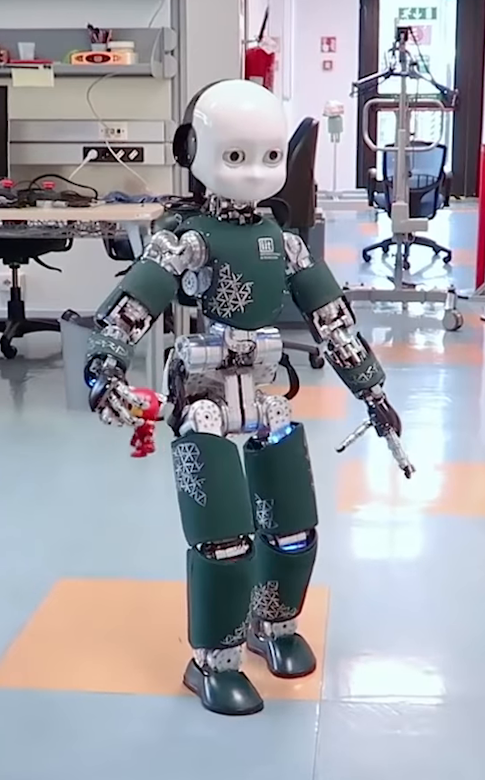
\includegraphics[width=\columnwidth]{chapter_simplified_benchmarking/figures/step1.png}
    \end{subfigure}
    \hfill
           \begin{subfigure}[b]{0.32\textwidth}
        \centering
        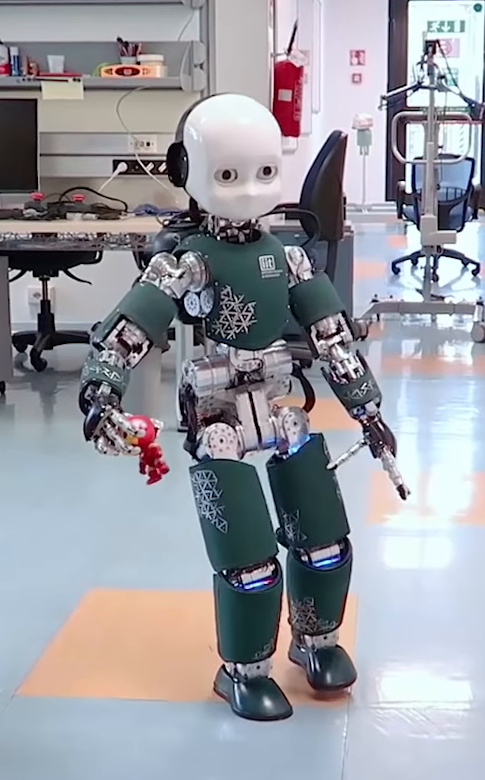
\includegraphics[width=\columnwidth]{chapter_simplified_benchmarking/figures/step2.png}
    \end{subfigure}
    \hfill
           \begin{subfigure}[b]{0.32\textwidth}
        \centering
        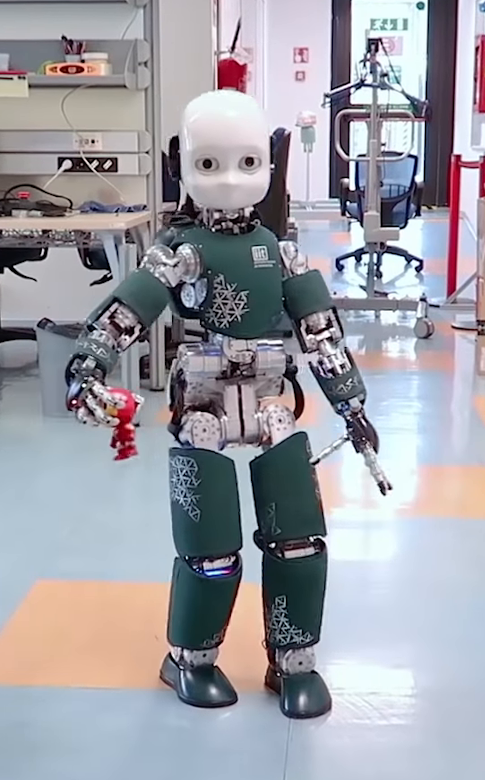
\includegraphics[width=\columnwidth]{chapter_simplified_benchmarking/figures/step3.png}
    \end{subfigure}
    \caption{The iCub robot walks with the 3 layer controller architecture of Figure~\ref{fig:three-layer-simplified-benchmarking}.}
    \label{fig:icub_walking_simplified}
\end{figure}

\section{Results}
\label{sec:results_simplified_benchmarking}
In this section, we present experiments obtained with several implementations of the simplified model controllers, namely: the \emph{instantaneous} and the \emph{predictive} controllers.

To benchmark the different simplified model controllers, we test the algorithms on the iCub humanoid robot v2.7 -- Section~\ref{sec:icub2.7}. We attach the simplified control layer to the three-layer controller architecture shown in Figure~\ref{fig:three-layer}. In this framework, the whole-body control layer implements the kinematics-based whole-body QP presented in section~\ref{sec:ik_qp}. Figure~\ref{fig:icub_walking_simplified} shows the humanoid robot iCub walking with the simplified models controller presented in this chapter.

The control architecture runs on the iCub head's computer, namely a 4-th generation Intel \textsuperscript{\tiny\textregistered} Core i7 @ $\SI{1.7}{\giga \hertz}$. In any of its implementations, the architecture takes (on average) less than $\SI{3}{\milli \second}$ to evaluate its output. The code is open source completely developed in C++: \href{https://github.com/robotology/walking-controllers}{\texttt{https://github.com/robotology/walking-controllers}}. The MPC problem presented in Section~\ref{predictive-control} is solved using the OSQP~\citep{Stellato2018} library~\footnote{Since our code is  written in pure C++, the QP problem is written by means of \texttt{osqp-eigen} a C++ wrapper for OSQP \href{https://github.com/robotology/osqp-eigen}{\texttt{https://github.com/robotology/osqp-eigen}}}.


Table~\ref{tab:max_velocity} summarizes the maximum velocities achieved using the different implementations of the control architecture. In particular, the labels \emph{instantaneous} and \emph{predictive} mean that the associated layer generates its output considering inputs and references either at the single time $t$ or for a time window, respectively. The labels, \emph{velocity} and \emph{position} control, instead, mean that the layer outputs are either desired joint velocities or position, respectively -- see Section~\ref{subsubsec-pos-vel-control}. 

\begin{table}[b]
    \centering
    \caption{Maximum forward straight walking velocities achieved using different implementations of the control architecture.
    }
    \begin{tabular}{cc|c}
         \begin{tabular}{@{}c@{}}Simplified Model  Control\end{tabular} &
         \begin{tabular}{@{}c@{}}Whole-Body QP Control\end{tabular} &
         \begin{tabular}{@{}c@{}}Max Straight Velocity (m/s)\end{tabular}\\
        \hline
        Predictive  & Velocity  &  0.1563\\
        Predictive  & Position  & 0.1645\\
        Instantaneous  & Velocity  &  0.1809\\
        Instantaneous  & Position  & 0.3372
    \end{tabular}
    \label{tab:max_velocity}
\end{table}

Let us remark that all the implemented control architectures exploit the controller presented in Section~\ref{ZMP-CoM-Controller} to attempt the stabilization of the desired center of pressure and desired center of mass position and velocity. The performance of this controller is highly dependent on the gains $K_{zmp}$ and $K_{com}$. In particular, we observed that the gains in achieving good tracking during standing and walking were not the same. For this reason, we implemented a gain-scheduling technique depending on whether the robot is walking or standing. The transition between the two sets of gains is smoothed with a minimum jerk trajectory \citep{Pattacini2010}.


To compare the simplified models controllers, we decided to perform two main experiments. These two experiments represent the maximum robot velocity that has been achieved with all architectures and the maximum velocity achieved with a specific architecture only -- see Table~\ref{tab:max_velocity}. That is, 
\begin{itemize}
    \item[-] \textbf{Experiment 1}: a forward robot speed of $\SI{0.1563}{\meter \per \second}$;
    \item[-] \textbf{Experiment 2}: a forward robot speed of $\SI{0.3372}{\meter \per \second}$.
\end{itemize}

\begin{figure}[t]
    \centering
    \begin{myframe}{Instantaneous + Position Control}
        \centering
    \begin{subfigure}[b]{0.49\textwidth}
        \centering
        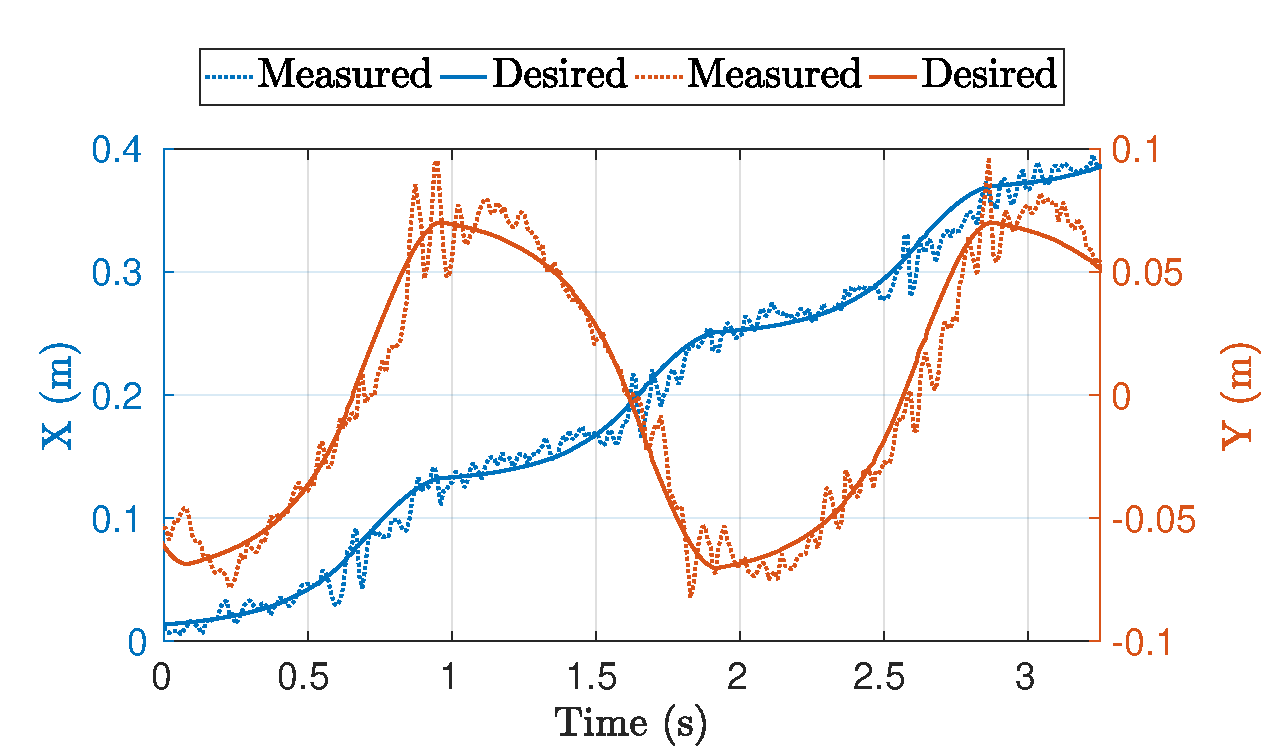
\includegraphics[width=\textwidth]{chapter_simplified_benchmarking/figures/inst_pos-min_vel-dcm.pdf}
        \caption{DCM}
        \label{fig:inst_pos-min_vel-dcm}
    \end{subfigure}
    \hfill
    \begin{subfigure}[b]{0.49\textwidth}
        \centering
        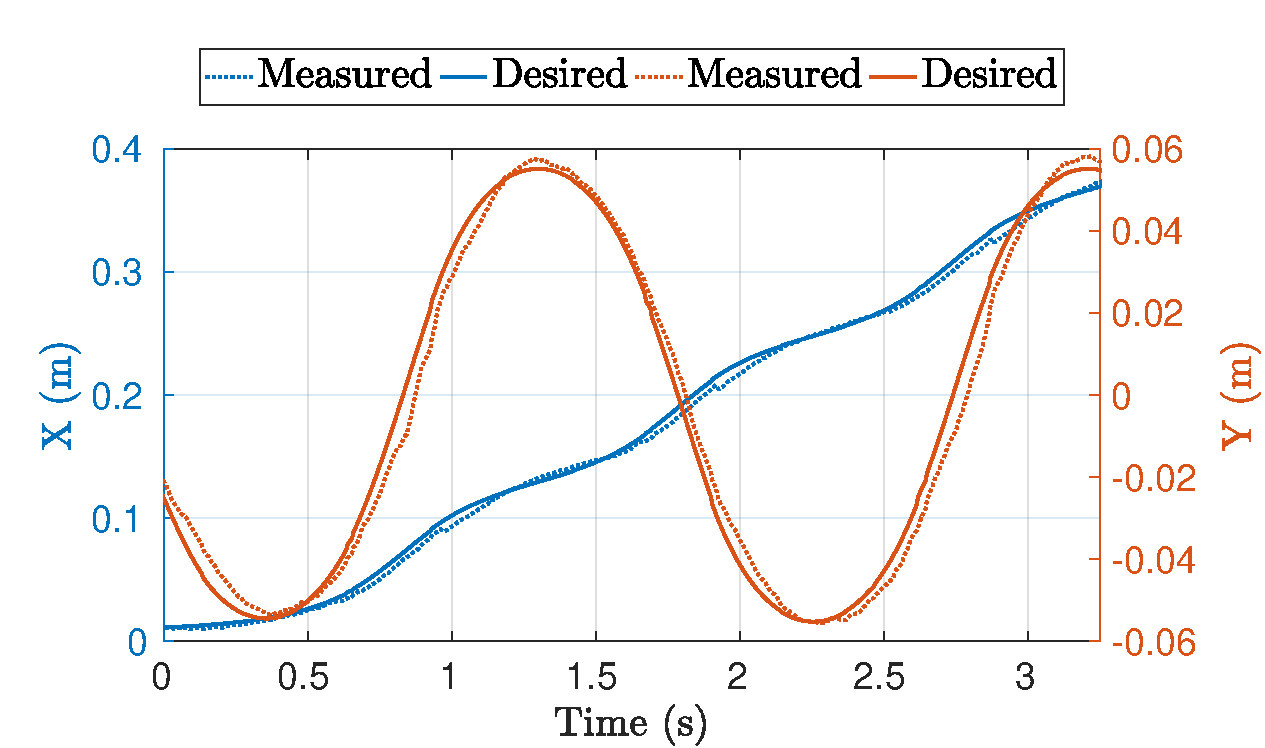
\includegraphics[width=\textwidth]{chapter_simplified_benchmarking/figures/inst_pos-min_vel-com.pdf}
        \caption{CoM}
        \label{fig:inst_pos-min_vel-com}
    \end{subfigure}
    \hfill
    \begin{subfigure}[b]{0.49\textwidth}
        \centering
        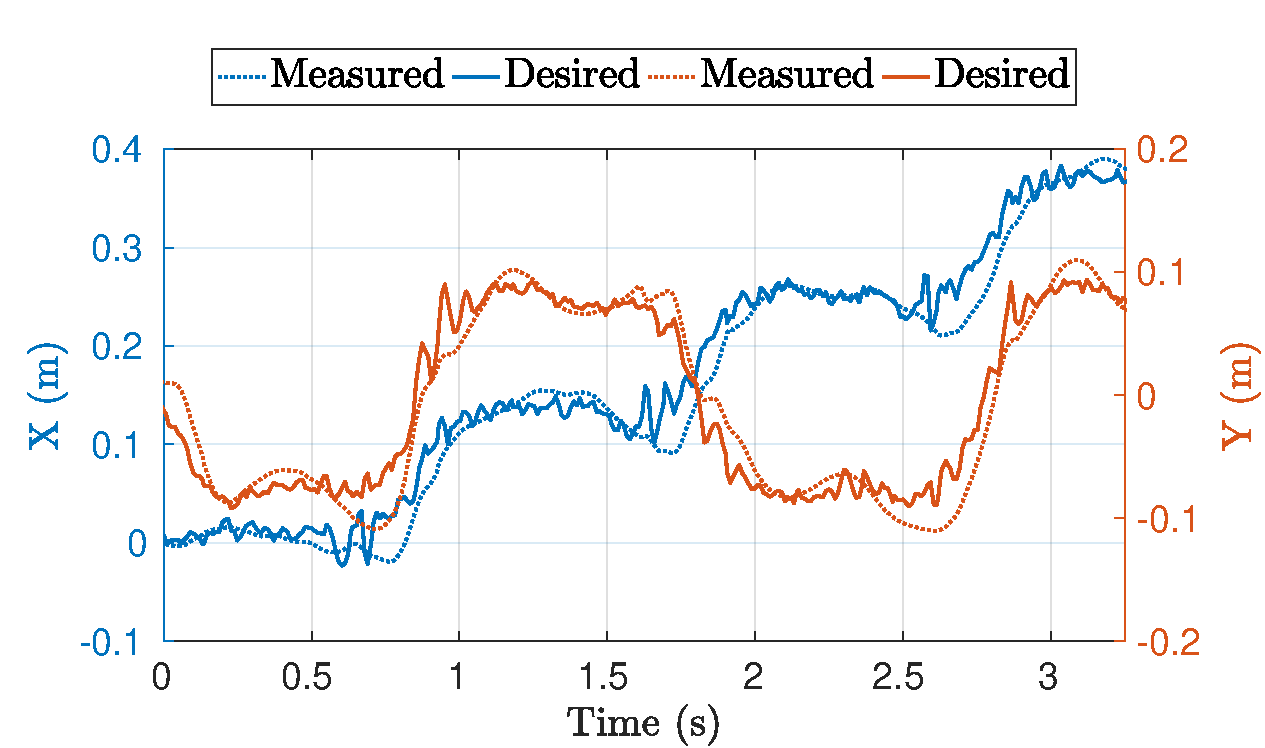
\includegraphics[width=\textwidth]{chapter_simplified_benchmarking/figures/inst_pos-min_vel-zmp.pdf}
        \caption{ZMP}
        \label{fig:inst_pos-min_vel-zmp}
    \end{subfigure}
    \end{myframe}
    \caption{Tracking of the DCM (a), CoM (b) and ZMP (c) using the instantaneous controller with the whole-body controller as position control. Walking velocity:  $\SI{0.19}{\meter \per \second}$.}
\end{figure}

\begin{figure}[t]
    \begin{myframe}{Predictive + Position Control}
     \centering
    \begin{subfigure}[b]{0.49\textwidth}
        \centering
        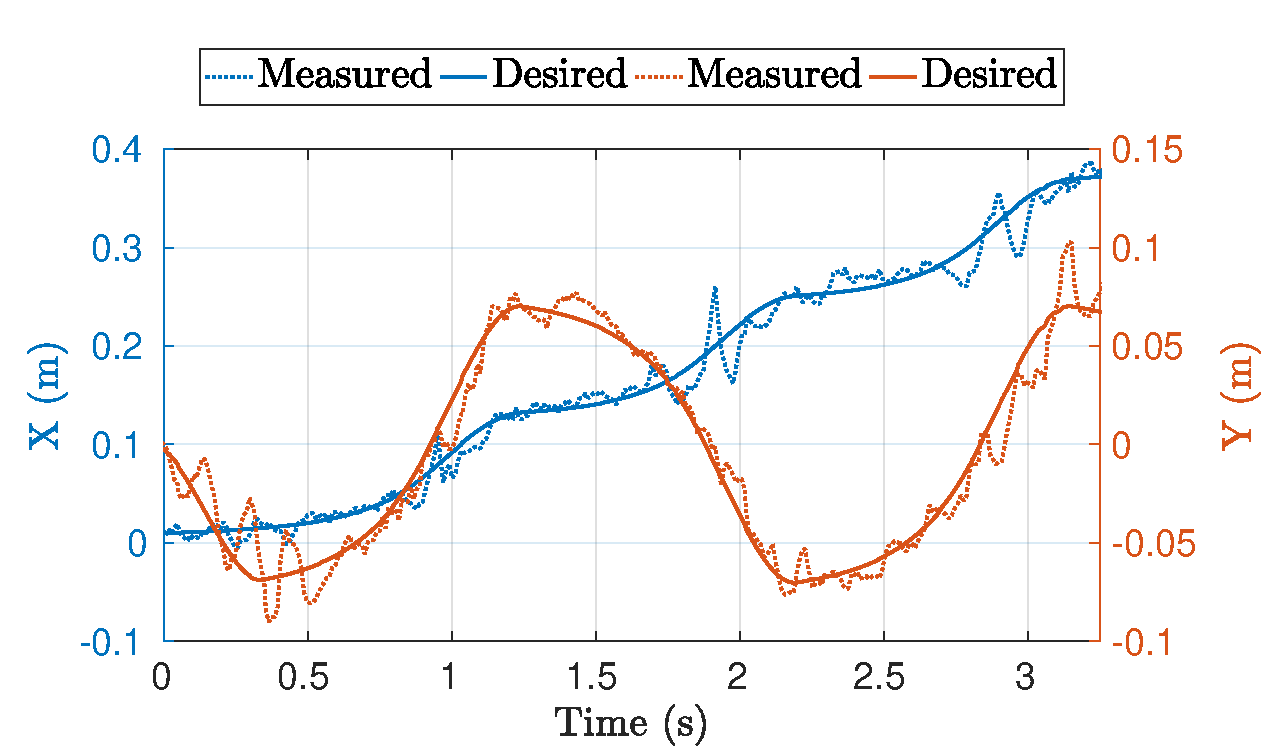
\includegraphics[width=\textwidth]{chapter_simplified_benchmarking/figures/mpc_pos-min_vel-dcm.pdf}
        \caption{DCM}
        \label{fig:mpc_pos-min_vel-dcm}
    \end{subfigure}
    \hfill
    \begin{subfigure}[b]{0.49\textwidth}
        \centering
        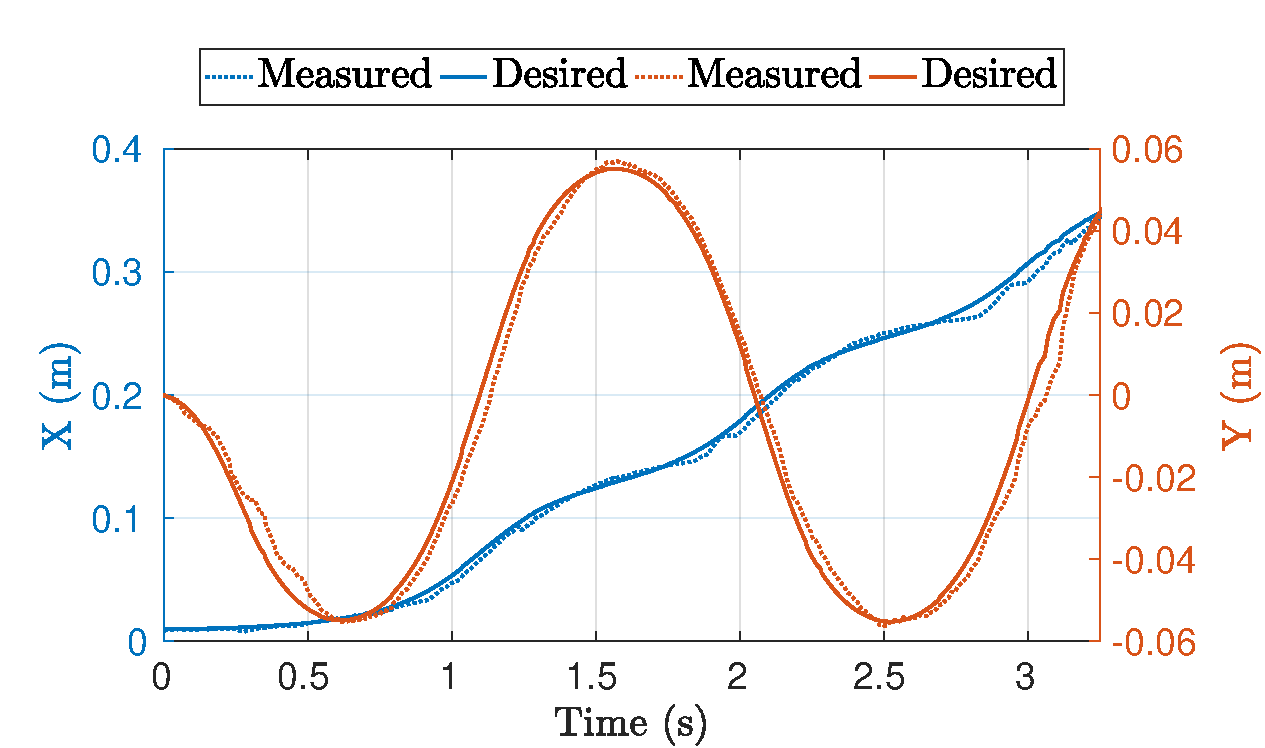
\includegraphics[width=\textwidth]{chapter_simplified_benchmarking/figures/mpc_pos-min_vel-com.pdf}
        \caption{CoM}
        \label{fig:mpc_pos-min_vel-com}
    \end{subfigure}
         \begin{subfigure}[b]{0.49\textwidth}
        \centering
        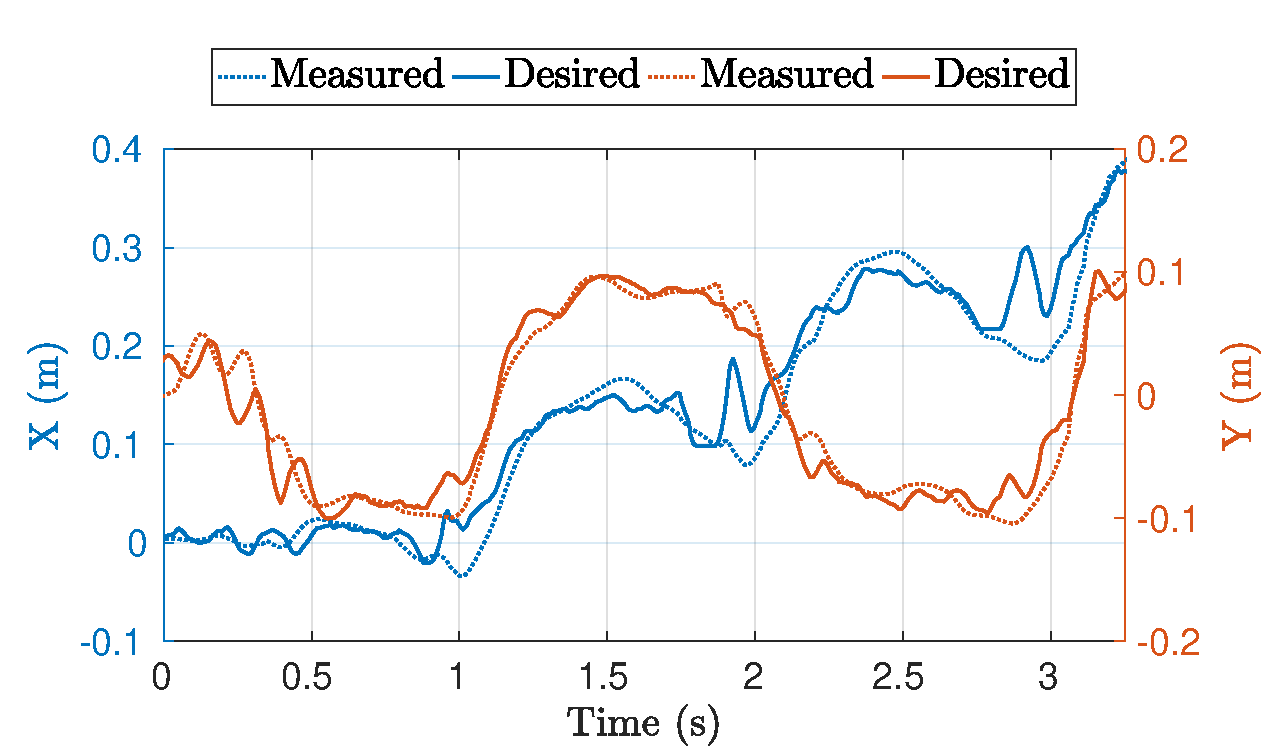
\includegraphics[width=\textwidth]{chapter_simplified_benchmarking/figures/mpc_pos-min_vel-zmp.pdf}
        \caption{ZMP}
        \label{fig:mpc_pos-min_vel-zmp}
    \end{subfigure}
    \end{myframe}
    \caption{Tracking of the  DCM (a), CoM (b) and ZMP (c) using the MPC and the whole-body controller as position control. Walking velocity:  $\SI{0.19}{\meter \per \second}$.}
\end{figure}
\begin{figure}[t]
     \vspace*{-0.1cm}
    \begin{myframe}{Instantaneous + Position Control}
    \centering
        \begin{subfigure}[b]{0.49\textwidth}
        \centering
        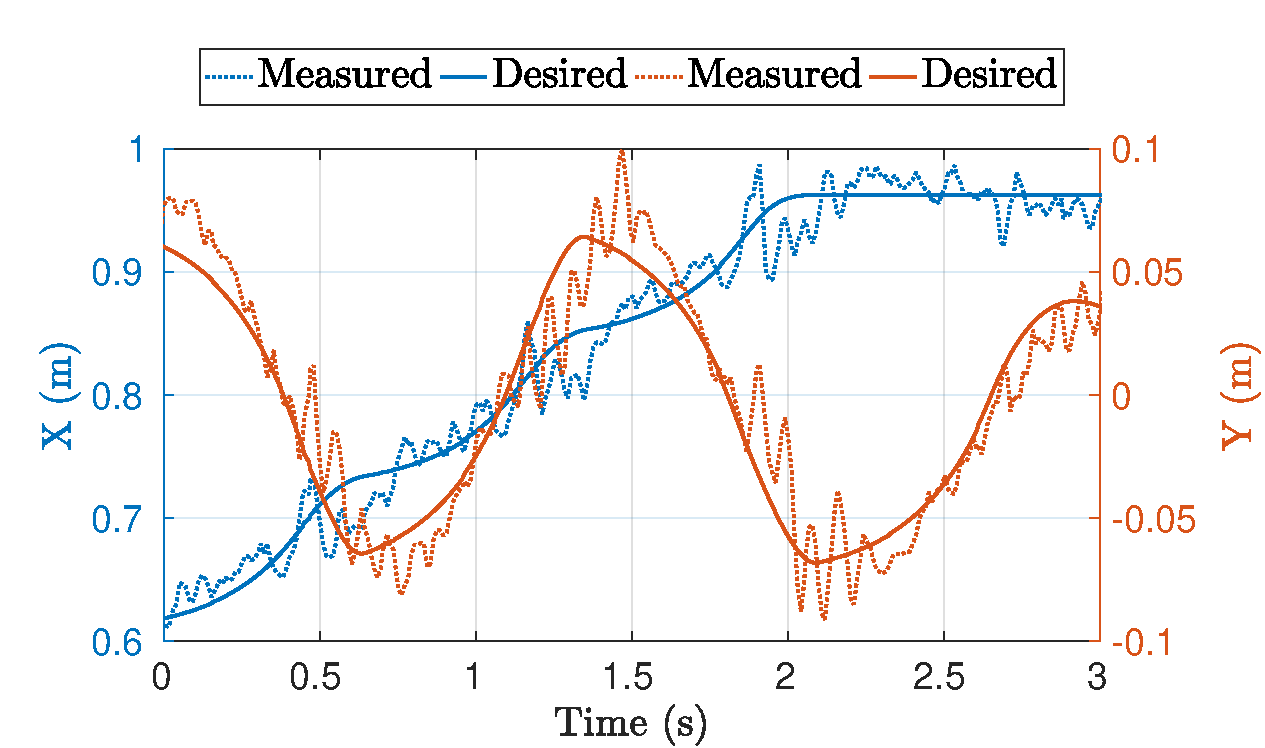
\includegraphics[width=\textwidth]{chapter_simplified_benchmarking/figures/inst_pos-max_vel-dcm.pdf}
        \caption{DCM}
        \label{fig:inst_pos-max_vel-dcm}
    \end{subfigure}
    \hfill
     \begin{subfigure}[b]{0.49\textwidth}
        \centering
        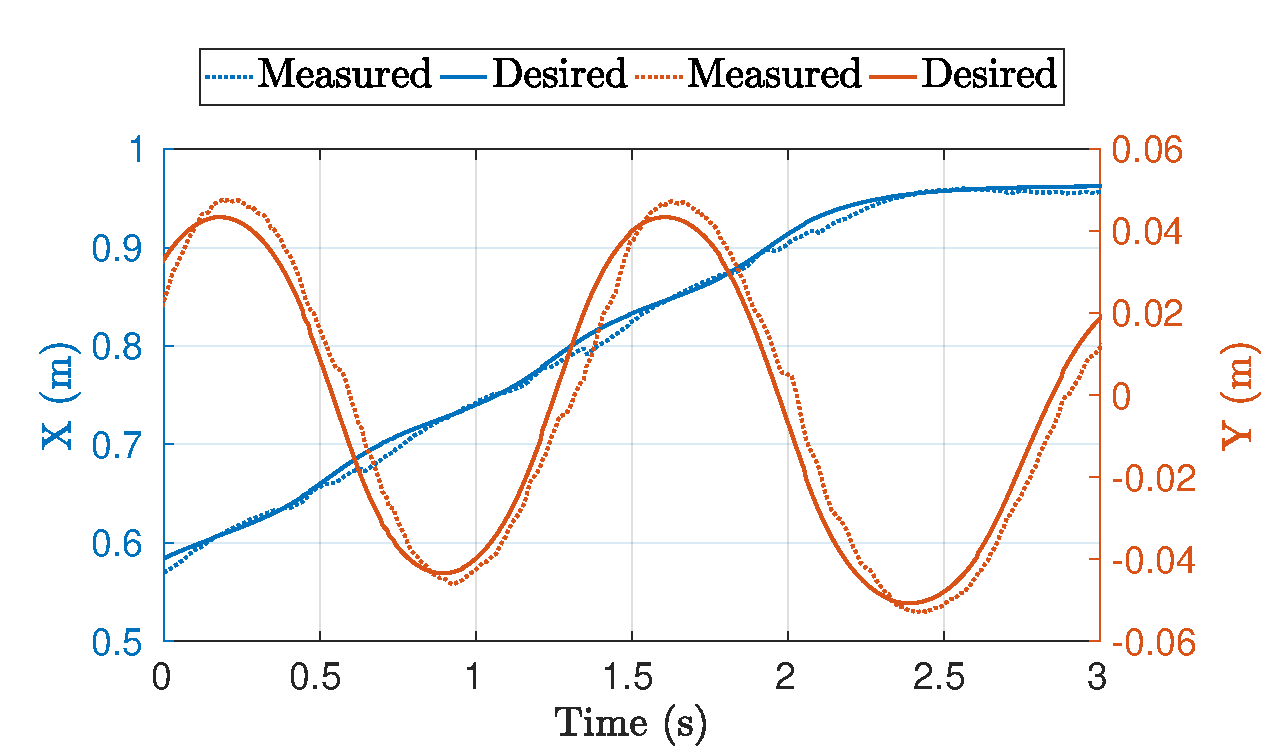
\includegraphics[width=\textwidth]{chapter_simplified_benchmarking/figures/inst_pos-max_vel-com.pdf}
        \caption{CoM}
        \label{fig:inst_pos-max_vel-com}
    \end{subfigure}
    \hfill
    \begin{subfigure}[b]{0.49\textwidth}
        \centering
        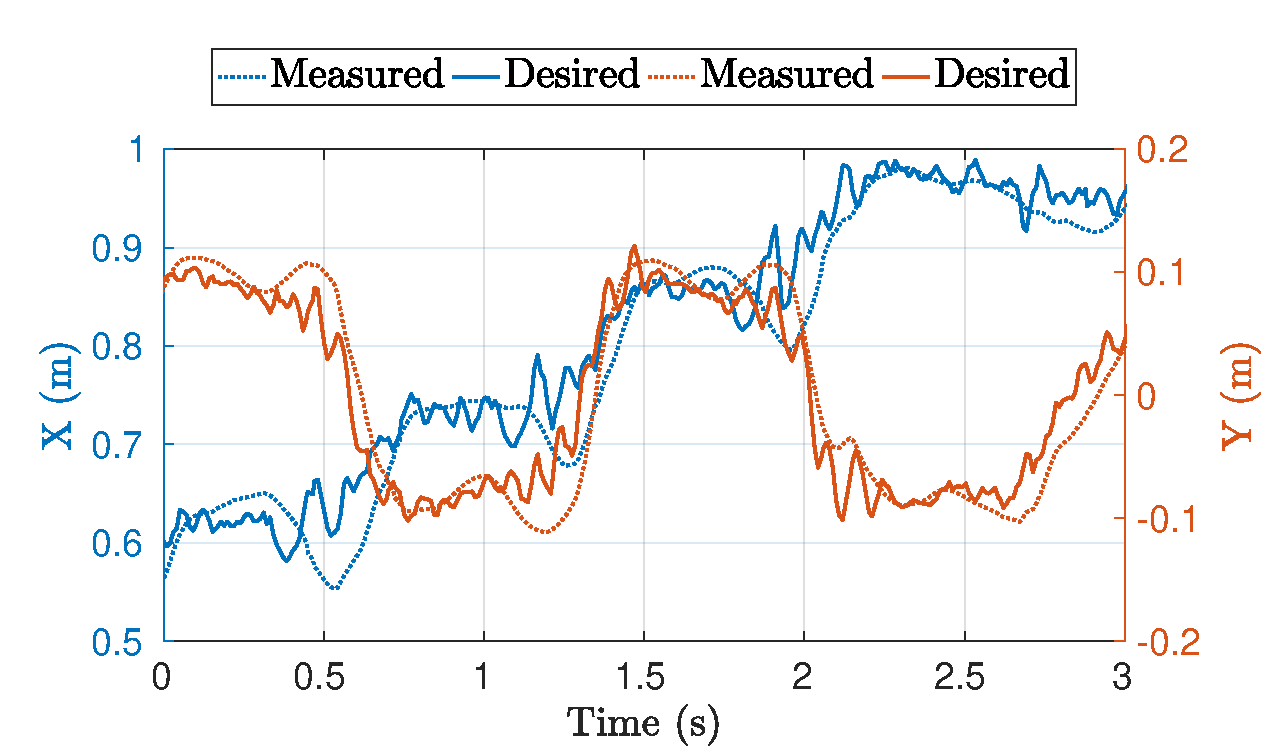
\includegraphics[width=\textwidth]{chapter_simplified_benchmarking/figures/inst_pos-max_vel-zmp.pdf}
        \caption{ZMP}
        \label{fig:inst_pos-max_vel-zmp}
    \end{subfigure}
    \end{myframe}
    \caption{Tracking of the DCM (a), CoM (b) and ZMP (c) with the instantaneous and whole-body QP control as position.  Walking velocity: $\SI{0.41}{\meter \per \second}$.}
\end{figure}
\begin{figure}[t]
    \begin{myframe}{Predictive + Position Control}
    \centering
    \begin{subfigure}[b]{0.49\textwidth}
        \centering
        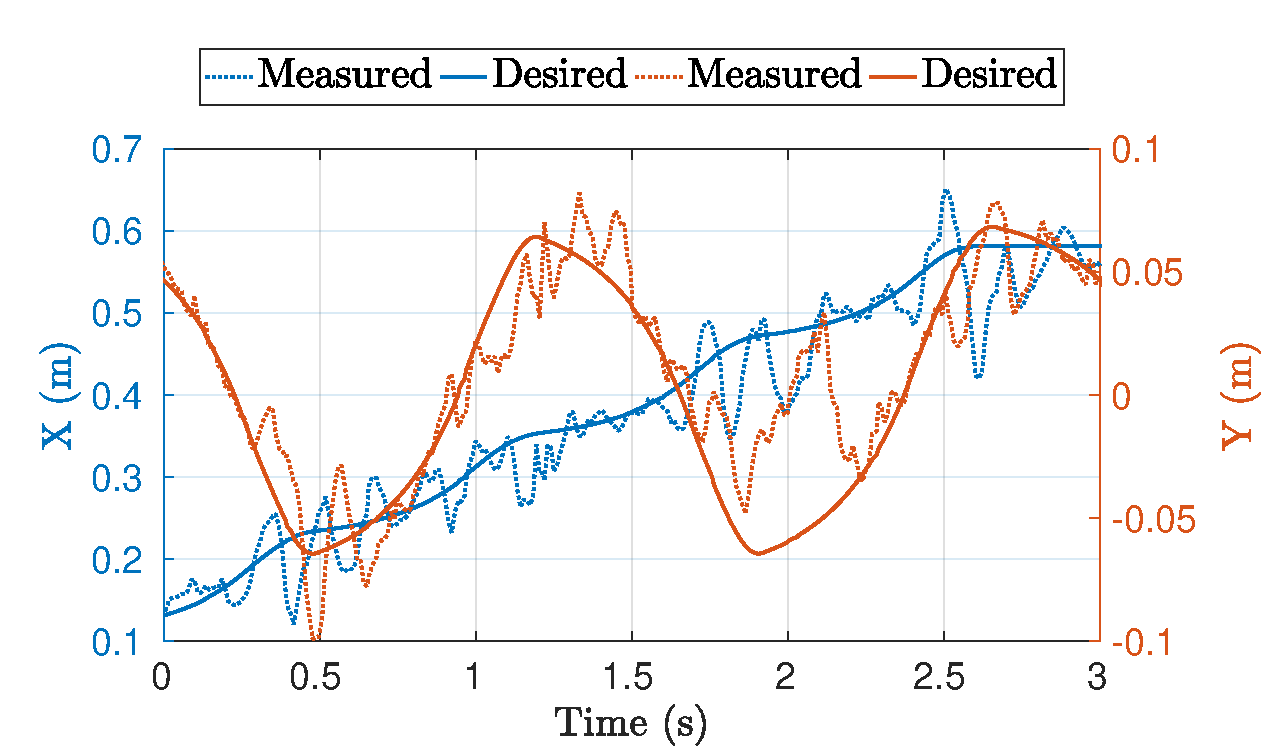
\includegraphics[width=\textwidth]{chapter_simplified_benchmarking/figures/mpc_pos-max_vel-dcm.pdf}
        \caption{DCM}
        \label{fig:mpc_pos-max_vel-dcm}
    \end{subfigure}
    \hfill
     \begin{subfigure}[b]{0.49\textwidth}
        \centering
        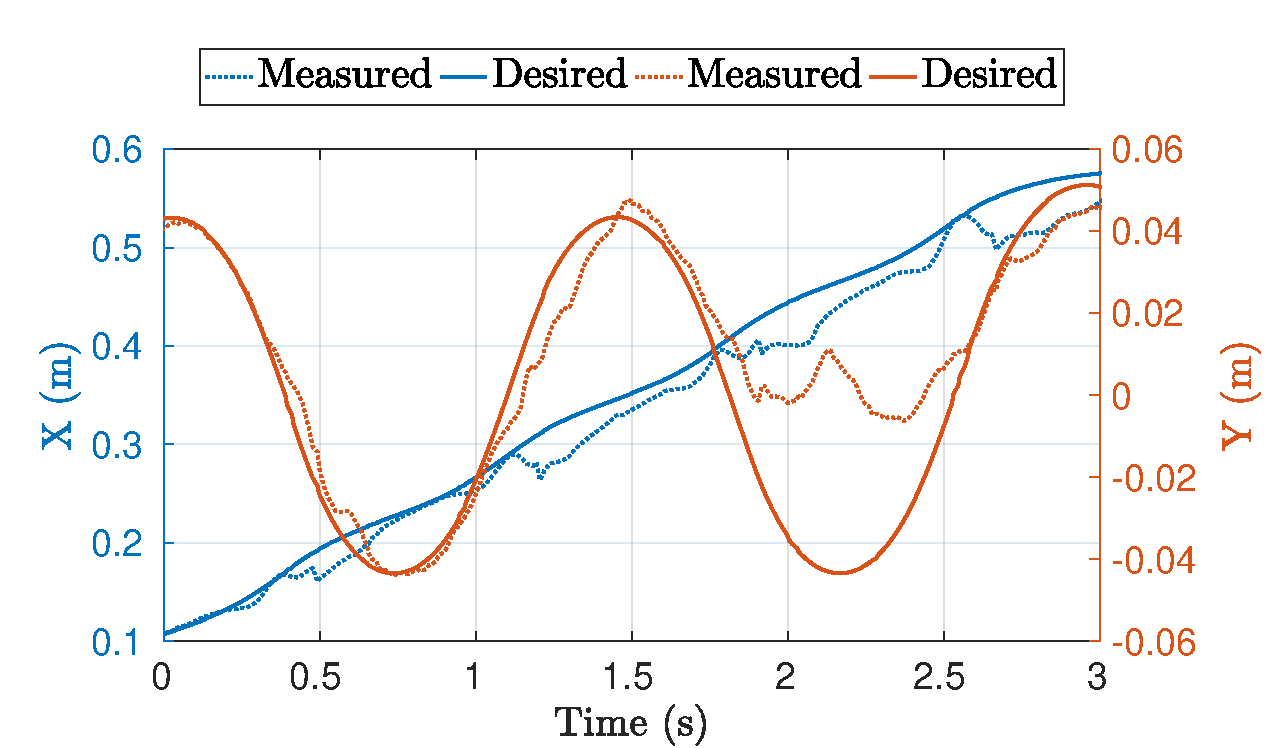
\includegraphics[width=\textwidth]{chapter_simplified_benchmarking/figures/mpc_pos-max_vel-com.pdf}
        \caption{CoM}
        \label{fig:mpc_pos-max_vel-com}
    \end{subfigure}
    \hfill
    \begin{subfigure}[b]{0.49\textwidth}
        \centering
        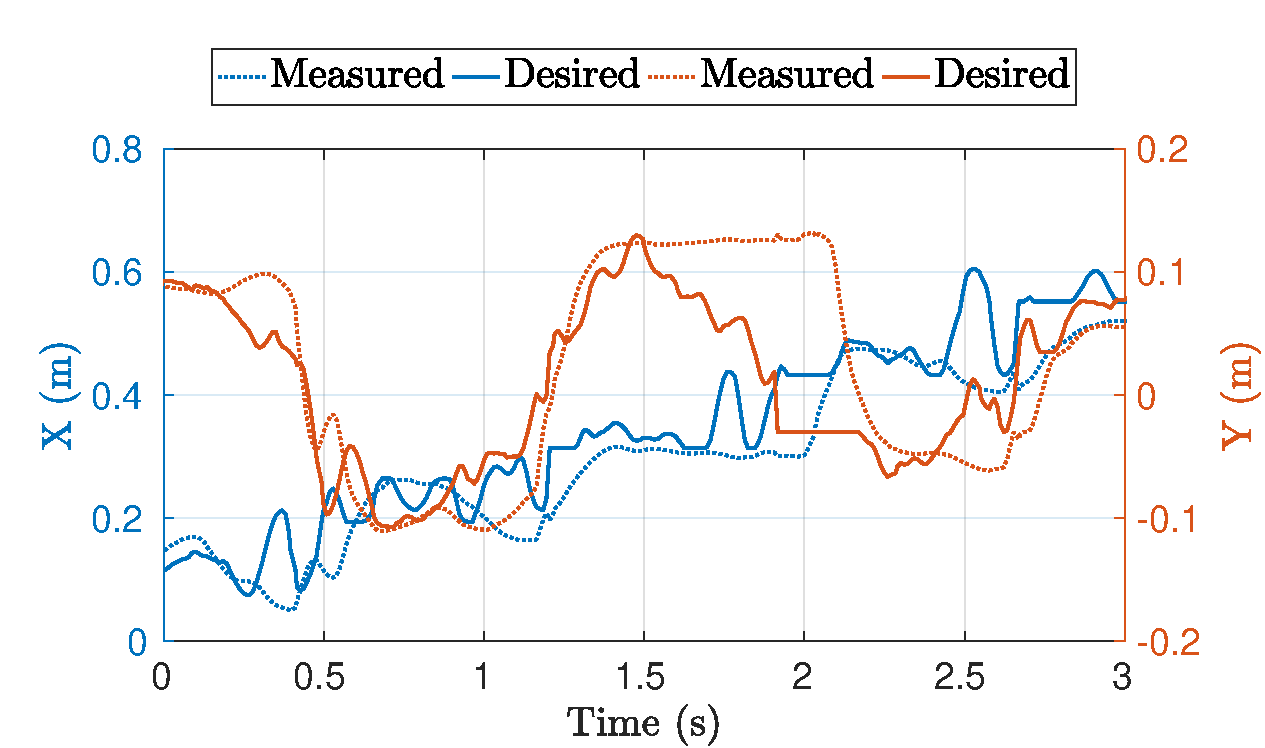
\includegraphics[width=\textwidth]{chapter_simplified_benchmarking/figures/mpc_pos-max_vel-zmp.pdf}
        \caption{ZMP}
        \label{fig:mpc_pos-max_vel-zmp}
    \end{subfigure}
    \end{myframe}
    \caption{Tracking of the  DCM (a), CoM (b) and ZMP (c) with the predictive and whole-body QP control as position control. At $t\approx \SI{2}{\second}$, the robot falls down.  Walking velocity: $\SI{0.41}{\meter \per \second}$.}
    \vskip-0.5cm
\end{figure}

We compare the control laws~\eqref{eq:reactive_dcm} and~\eqref{eq:mpc_solution_simplified}, which both generate a (desired) center of pressure that attempts to stabilize the desired DCM. To simplify the comparison, the controller of the \emph{whole-body QP layer} is kept fixed in this section, and we show and discuss only the results when the robot is position controlled. A complete comparison of the kinematics-based whole-body controllers is presented in Section~\ref{sec:wbc_experimental_results}.
In the following experiments, we set the time horizon of the predictive control to $\SI{2}{\second}$.

\subsection{Experiment 1: a forward robot speed of 0.1563 m s$^{\text{-1}}$}
Figures \ref{fig:inst_pos-min_vel-dcm} and \ref{fig:mpc_pos-min_vel-dcm} show the DCM tracking performances obtained with the instantaneous and predictive controllers, respectively. Both controllers seem to show good tracking performances, and the DCM error is kept below $\SI{5}{\centi \meter}$ in both cases. Note, however, that the instantaneous controller induces faster variations of the measured DCM. This contributes to the overall higher vibrations of the robot. One of the reasons for this variation is that the instantaneous controller~\eqref{eq:reactive_dcm} injects a (desired) center of pressure proportional to the measured DCM, which in turn contains the center of mass velocity. To mitigate this, we may filter the joint velocities appropriately. However, in our case, the joint velocities were not filtered to avoid delays in the measured DCM. Our experience showed that adding a filter to joint velocities is not an easy task, and we did not find the right trade-off for obtaining overall performance improvements. 

Figures~\ref{fig:inst_pos-min_vel-com} and \ref{fig:mpc_pos-min_vel-com} present CoM tracking performances, which are mainly dependent on the ZMP-CoM controller~\eqref{eq:ZMP_controller}. This controller receives the desired DCM values from the \emph{simplified model control} layer, which are obtained with the instantaneous or predictive controllers. In both cases, the CoM error is kept below $\SI{2}{\centi \meter}$. Figures~\ref{fig:inst_pos-min_vel-zmp} and~\ref{fig:mpc_pos-min_vel-zmp} represent the ZMP tracking performance, which is still mainly dependent on the ZMP-CoM controller~\eqref{eq:ZMP_controller}. It is important to note that the desired ZMP is smoother when the \emph{simplified model control} uses the predictive law~\eqref{eq:mpc_solution_simplified} to generate it. Indeed, this is a tunable property that depends on the associated weight in the cost function of the MPC problem. Although this smoother behavior contributes to less robot vibrations, overall robot performance became less reactive and, consequently, less robust to robot falls. Although the extensive hand-made tuning, we were not able to increase the robot velocity when the \emph{simplified model control} used the predictive law~\eqref{eq:mpc_solution_simplified}. 

\subsection{Experiment 2: a forward robot speed of 0.3372 m s$^{\text{-1}}$}
At a robot's desired walking speed of $\SI{0.3372}{\meter \per \second}$, there is initially no significant difference between the DCM tracking obtained with instantaneous and predictive control laws -- see Figures~\ref{fig:mpc_pos-max_vel-dcm} and~\ref{fig:inst_pos-max_vel-dcm} for $t < \SI{1.5}{\second}$. However, fast robot walking velocities require fast variations of the desired CoM and ZMP. This fast variation degrades the performance of the predictive controller around $t = \SI{1.5}{\second}$ -- see Figure~\ref{fig:mpc_pos-max_vel-zmp}. Clearly, these bad performances, in turn, induce poor tracking of the DCM shown in Figure~\ref{fig:mpc_pos-max_vel-dcm} at $t\approx \SI{2}{\second}$, and consequently the robot falls. At this point, one is tempted to increase the gain $K_\text{ZMP}$ of the controller~\eqref{eq:ZMP_controller}, which shall induce a better tracking of the ZMP. Unfortunately, this leads to higher robot oscillations induced by the noise on the estimated ZMP. And, as a consequence, the robot falls. 

We can conclude that the \emph{predictive simplified control} is much less robust than the \emph{instantaneous simplified control} with respect to ZMP tracking errors. Adding a low-pass filter to the ZMP measurement may improve the overall performance. However, in our case, adding filters led to slower system response and, consequently, to the robot falling.



\section{Conclusions \label{sec:conclusions_flexible_joint}}
This chapter presents the design of a whole-body QP control layer for a humanoid robot affected by link flexibility. We model the flexibility by introducing equivalent passive joints that simulate the motion caused by the link deformation.
We then considered the passive joints position and velocity as state of the floating base system dynamics. Thanks to this choice, we develop a whole-body controller that implicitly considers the joint flexibility in the stabilization problem. 
The chapter also details the design of an estimator that aims at computing the flexible joint state in real-time. 
\par
The proposed approach is validated in a simulated version of the TALOS humanoid robot, where its hip flexibility has a significant impact while performing locomotion tasks. Moreover, the architecture is then compared with a whole-body controller that considers all links of the robot rigid.
\par
As a future work, we plan to mitigate the discontinuity of the contact forces by performing a smother transition between contiguous support phases. We also plan to make a detailed comparison with other state-of-the-art controllers that
consider the flexibility of the robot link~\citep{Villa2022TorqueFlexibility}. In addition, we plan to validate the architecture on the real robot.


